\documentclass[a4paper]{article}
\usepackage[14pt]{extsizes} % для того чтобы задать нестандартный 14-ый размер шрифта
\usepackage[utf8]{inputenc}
\usepackage[english, russian]{babel}
\usepackage{setspace,amsmath}
\usepackage{epigraph} % для эпиграфов и продвинутых цитат
\usepackage{csquotes} % ещё одна штука для цитат
\usepackage[unicode, pdftex]{hyperref} % подключаем hyperref (для ссылок внутри  pdf)
\usepackage{amssymb} % в том числе для красивого знака пустого множества
\usepackage{amsthm} % в т.ч. для оформления доказательств
\usepackage[left=20mm, top=15mm, right=15mm, bottom=15mm, footskip=7mm]{geometry} % настройки полей документа 
\usepackage[active]{srcltx}
\usepackage{indentfirst}
\usepackage{listings}
\usepackage{tocloft}
\usepackage{misccorr} 
\usepackage{graphicx}
\usepackage{caption}
\usepackage[style=numeric,sorting=none]{biblatex}
\DeclareCaptionLabelSeparator{defffis}{ --- }
\captionsetup{justification=centering,labelsep=defffis}
\graphicspath{{images/}}
\DeclareGraphicsExtensions{.jpg}
\renewcommand{\cftsecleader}{\cftdotfill{\cftsubsecdotsep}}
\newcommand{\ran}{{\rm ran}\,}
\newcommand{\diag}{{\rm diag}\,}
% переименовываем  список литературы в "список используемой литературы"
\addto\captionsrussian{\def\refname{Список используемой литературы}}
\addto\captionsrussian{\renewcommand\listfigurename{Список рисунков}}
\newcounter{totreferences}
\pretocmd{\bibitem}{\addtocounter{totreferences}{1}}{}{}
\newtheorem{theorem}{Теорема} % задаём выводимое слово (для теорем)
\newtheorem{definition}{Опредление} % задаём выводимое слово (для определений) 
% объявляем новые команды 
\newcommand{\RNumb}[1]{\uppercase\expandafter{\romannumeral #1\relax}}

\begin{document} % начало документа
\def\figurename{Рисунок}

\makeatletter
\lst@UserCommand\lstlistlistingname{Список листингов кода:}
\makeatother
 
% НАЧАЛО ТИТУЛЬНОГО ЛИСТА
\begin{center}
 \hfill \break
\hfill\break
\hfill\break
\hfill \break
\hfill \break
\hfill \break
\hfill \break
\hfill \break
\hfill \break
\large{\textbf{CORPORATE FOOD CHECKER}}\\
\hfill \break
\hfill \break
\large{\textbf{Система выбора корпоративных обедов на предприятии}}\\
\large{\textbf{Инструкция пользователя}}\\
\hfill \break
\hfill \break
Версия 0.0.1\\
\hfill \break
\hfill \break
\hfill \break
\hfill \break
\hfill \break
\hfill \break
\hfill \break
\hfill \break
\hfill \break
\hfill \break
\hfill \break
\hfill \break
\hfill \break
\begin{center} Санкт-Петербург, 2020 \end{center}
\end{center}
\thispagestyle{empty}
 
% КОНЕЦ ТИТУЛЬНОГО ЛИСТА
 
\newpage 
	\addcontentsline{toc}{section}{Содержание} 
    \tableofcontents % Вывод содержания
\newpage

\section{Назначение и описание программы}

Программа предназначена для автоматизации выбора пользователями готовых обедов на предприятии. Она позволяет выбрать каждому из зарегистрированных пользователей один из нескольких вариантов обеда, доступных на выбранную дату, подтвердить свой выбор и сохранить его. Администратору приложения будет показан отчет на каждую дату, включающий общую статистику по выбранным пользователями обедам.

\section{Интерфейс программы и начало работы}

Интерфейс программы можно условно разделить на две части: простого пользователя и административную панель. При входе на главную страницу будет показано приветственное окно с названием программы и предложение войти под своей учетной записью. Интерфейс адаптивный - можно использовать его как на персональном компьютере с полноценным браузером, так и на мобильном телефоне с современной операционной системой (как Android, так и iOS). На рисунках ~\ref{fig:image1} и ~\ref{fig:image2} показаны внешний вид приложения на разных системах.

\begin{figure}[h]
\center{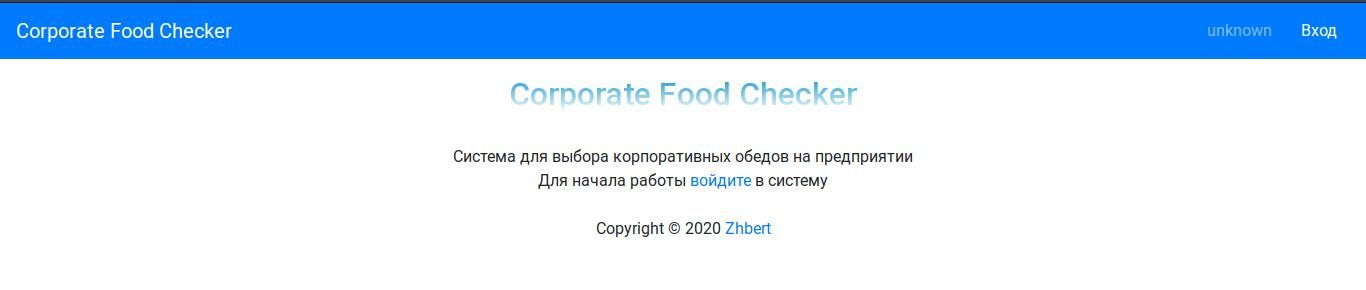
\includegraphics[width=1\linewidth]{001}}
\caption{Главная страница приложения}
\label{fig:image1}
\end{figure}

\begin{figure}[h]
\center{
\includegraphics[scale=0.23]{002}}
\caption{Главная страница приложения на мобильном устройстве}
\label{fig:image2}
\end{figure}

\section{Вход в систему}

Для входа в систему перейдите на страницу входа. Попасть на нее можно либо нажав на кнопку <<\textbf{Вход}>> в верхнем правом углу главного меню, либо пройдя по ссылке <<\textbf{войдите}>> на главной странице.

\begin{figure}[h]
\center{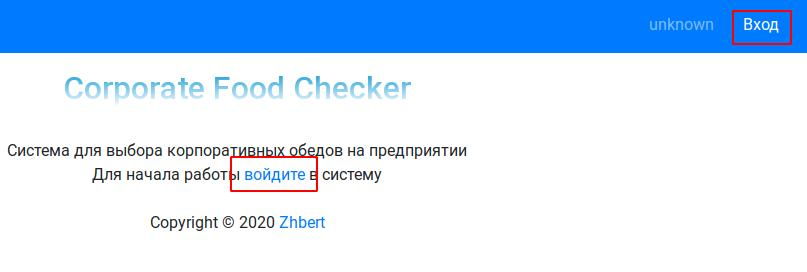
\includegraphics[width=1\linewidth]{003}}
\caption{Кнопка входа и ссылка на страницу входа}
\label{fig:image3}
\end{figure}

В мобильной версии программы кнопка \textbf{<<Вход>>} может быть скрыта в главном меню. Главное меню доступно по нажатию кнопки в верхнем правом углу экрана.

\begin{figure}[h]
\center{
\includegraphics[scale=0.5]{004}}
\caption{Главное меню и кнопка входа в мобильной версии}
\label{fig:image4}
\end{figure}

После нажатия кнопки произойдет переход на страницу входа в систему.

\begin{figure}[h]
\center{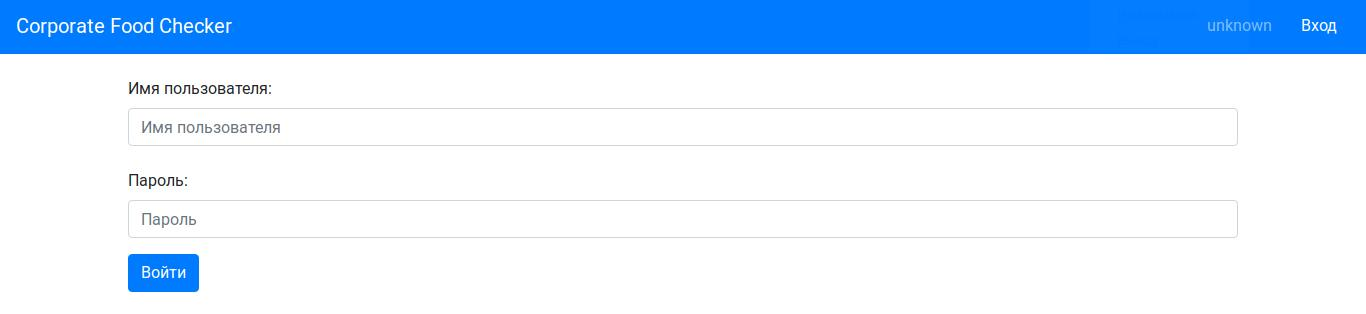
\includegraphics[width=1\linewidth]{005}}
\caption{Страница входа}
\label{fig:image5}
\end{figure}

Для входа введите свои учетные данные\footnote{\textbf{Обратите внимание!} Учетные данные главного администратора приложения выдаются разработчиком при передаче доступа к программе.}.

Введите имя пользователя и пароль в соответствующие поля и нажмите \textbf{<<Вход>>}. Если все прошло правильно, в правом верхнем углу возле кнопки \textbf{<<Вход>>} появится имя пользователя, а в главном меню появятся дополнительные пункты.

\begin{figure}[h]
\center{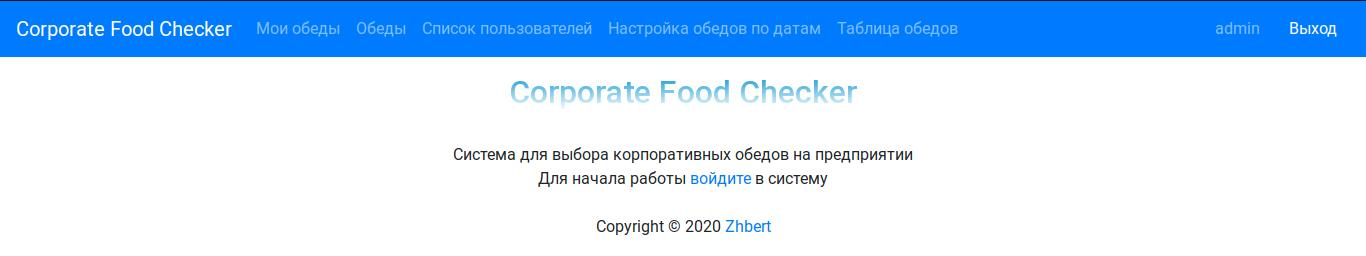
\includegraphics[width=1\linewidth]{006}}
\caption{Главная страница администратора системы}
\label{fig:image6}
\end{figure}

При неправильно введенных данных будет показано соответствующее сообщение об ошибке.

\begin{figure}[h]
\center{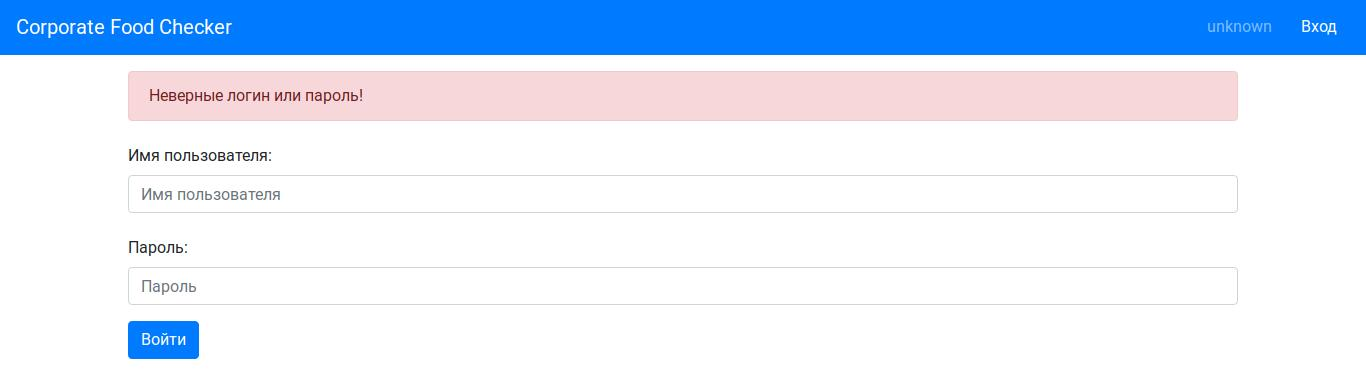
\includegraphics[width=1\linewidth]{007}}
\caption{Сообщение об ошибке входа в систему}
\label{fig:image7}
\end{figure}

\section{Администрирование системы}

\subsection{Алгоритм работы с системой}

Для правильной работы с системой следует выполнять действия в определенном порядке, представленном ниже\footnote{Выполнять действия именно в таком порядке следует только в первый раз. В дальнейшем возможно изменение порядка в зависимости от ситуации}.

\begin{itemize}
\setlength{\itemsep}{-2mm}
	\item \textbf{Создание пользователей} - создание учетных данных пользователей;
	\item \textbf{Создание обедов} - настройка комплексов обедов, доступных для заказа;
	\item \textbf{Настройка обедов по датам} -  присвоение соответствующих обедов конкретным датам;
\end{itemize}

\subsection{Создание и администрирование пользователей системы}

Для того, чтобы работники предприятия могли выбирать желаемые ими обеды, нужно создать для них учетные записи. Создание производит администратор системы на вкладке \textbf{<<Список пользователей>>}.

\begin{figure}[h]
\center{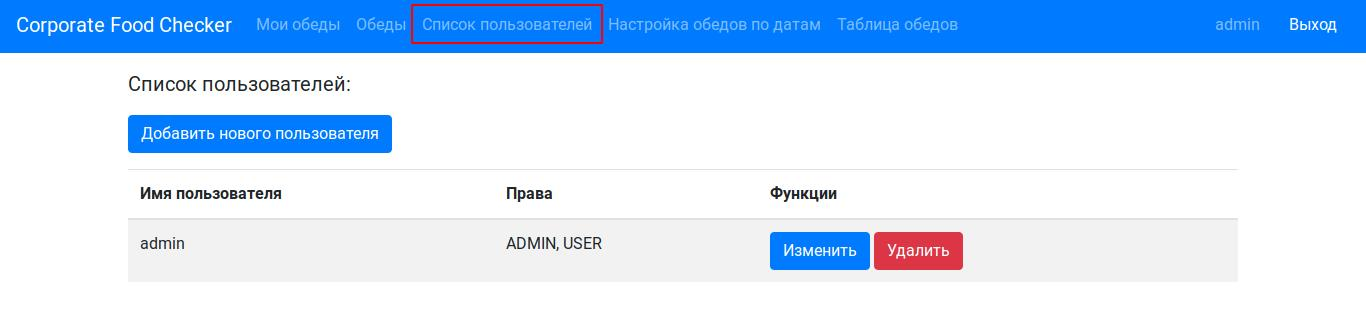
\includegraphics[width=1\linewidth]{008}}
\caption{Сообщение об ошибке входа в систему}
\label{fig:image8}
\end{figure}

Ручное создание учетных записей необходимо для точного соблюдения правильности подсчета: произвольная регистрация предоставит возможность создавать неактивные учетные данные или сделать их задвоение, что нарушит правильность статистики и при большом количестве пользователей будет выдавать достаточно большую погрешность.

На рисунке ~\ref{fig:image8} показана страница пользователей. В таблице представлены все пользователи системы. Таблица имеет три столбца:

\begin{itemize}
\setlength{\itemsep}{-2mm}
	\item \textbf{Имя пользователя} - имя пользователя, необходимое для входа в систему;
	\item \textbf{Права} - права пользователя в системе:
		\subitem \textbf{\textit{ADMIN}} -  администратор системы
		\subitem \textbf{\textit{USER}} - простой пользователь
	\item \textbf{Функции} -  действие, которые можно выполнить с учетной записью:
		\subitem \textbf{\textit{Изменить}} - изменение учетной записи;
		\subitem \textbf{\textit{Удалить}} - удаление учетной записи;
\end{itemize}

\subsubsection{Добавление нового пользователя}

Для добавления нового пользователя нужно нажать кнопку \textbf{<<Добавить нового пользователя>>} в верхней части страницы. При нажатии кнопки появится выпадающая форма для ввода данных нового пользователя.

\begin{figure}[h]
\center{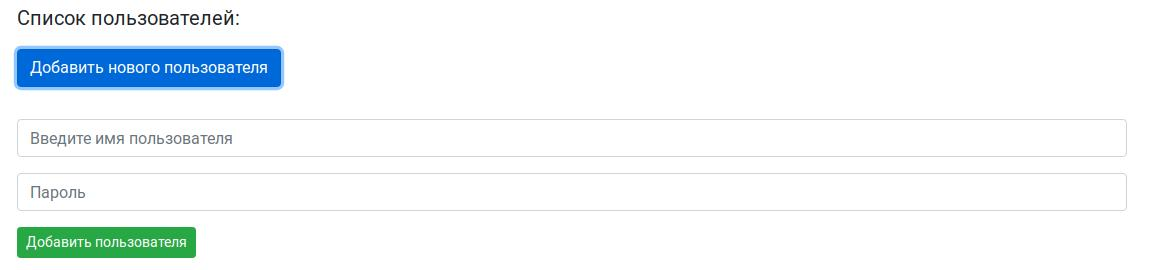
\includegraphics[width=1\linewidth]{009}}
\caption{Форма добавления нового пользователя}
\label{fig:image9}
\end{figure}

В соответствующие поля необходимо ввести имя пользователя и его пароль. Имя пользователя может быть как в английской раскладке, так и в русской, пароль же только на латинице. \textbf{Пробелы в имени пользователя недопустимы!}. Также обратите внимание, что после ввода пароль и сохранения данных \textbf{пароль просмотреть будет невозможно}, так как в базе данных он хранится не в явном виде, и вытащить его не представляется возможным. \textbf{Запоминайте или записывайте создаваемые пароли!} Для завершения операции нажмите кнопку \textbf{<<Добавить пользователя>>}

После успешного добавления пользователя произойдет перенаправление на страницу пользователей, в таблице которой появится только что созданный пользователь.

\begin{figure}[h]
\center{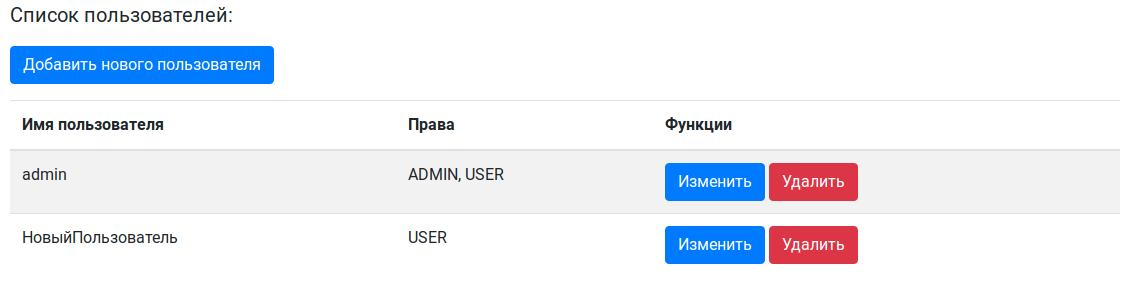
\includegraphics[width=1\linewidth]{010}}
\caption{Созданный новый пользователь}
\label{fig:image10}
\end{figure}

В случае неправильного ввода данных будет показана ошибка валидации данных.

\begin{figure}[h]
\center{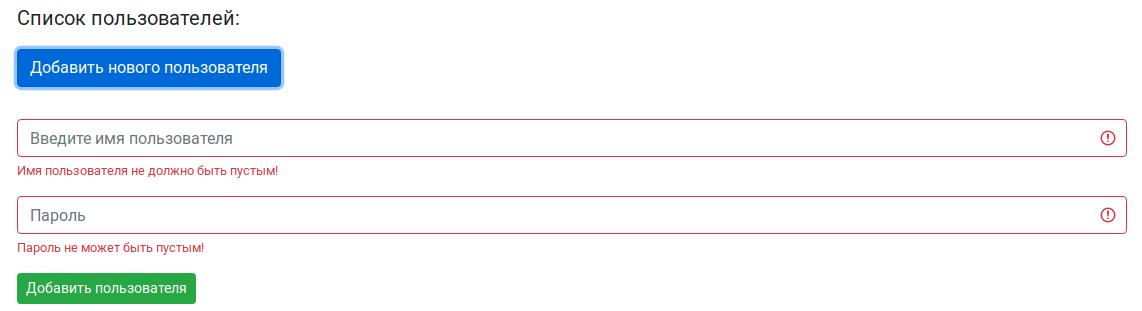
\includegraphics[width=1\linewidth]{011}}
\caption{Ошибка валидации}
\label{fig:image11}
\end{figure}

Права у нового пользователю по умолчанию стандартные - \textit{пользователь}. Для изменения роли пользователя в системе необходимо нажать кнопку \textbf{Изменить} в крайнем правом столбце соответствующей пользователю строки таблицы.

На открывшейся странице изменения пользователя можно выполнить следующие действия:

\begin{itemize}
\setlength{\itemsep}{-2mm}
	\item Изменить имя пользователя;
	\item Задать ему новый пароль\footnote{Старый пароль по описанным выше причинам не может быть применен автоматиески. Необходимо ввести пароль заново - либо новый, либо такой же, как был};
	\item Установить дополнительные права пользователя\footnote{Снимать галочку с прав USER не стоит, так как это может привести к неправильной работе системы} (ADMIN), если необходимо;
\end{itemize}

\begin{figure}[h]
\center{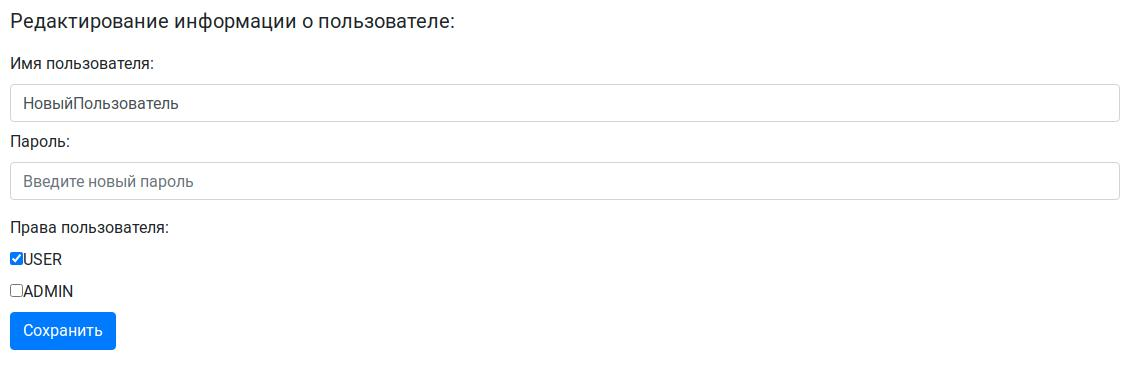
\includegraphics[width=1\linewidth]{012}}
\caption{Страница изменения учетной записи пользователя}
\label{fig:image12}
\end{figure}

Для завершения редактирования необходимо нажать кнопку \textbf{<<Сохранить>>}. В случае неправильно введенных данных на форме будет показано сообщение об ошибке.

\begin{figure}[h]
\center{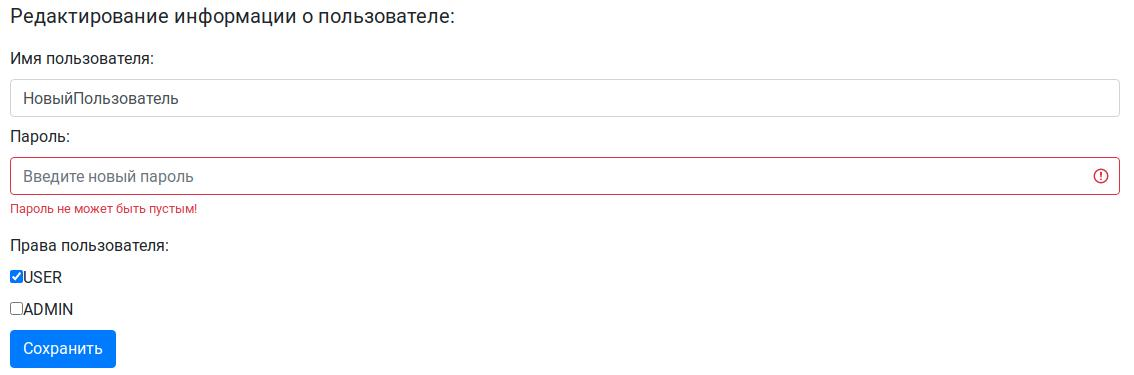
\includegraphics[width=1\linewidth]{013}}
\caption{Ошибка на странице изменения учетной записи}
\label{fig:image13}
\end{figure}

\newpage
\subsection{Администрирование обедов}

\subsubsection{Создание нового обеда}

Для того, чтобы система работала как нужно, необходимо создать комплексы обедов, доступные для выбора пользователями. Сделать это можно на странице \textbf{<<Обеды>>}. 

\begin{figure}[h]
\center{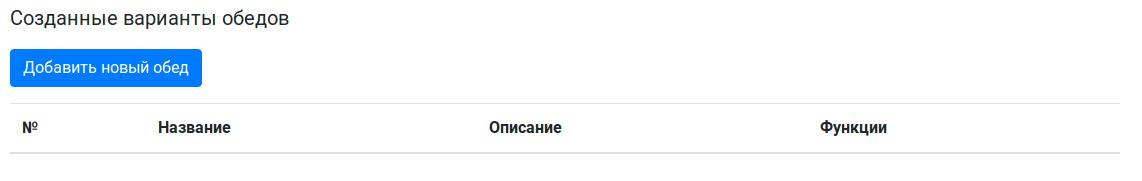
\includegraphics[width=1\linewidth]{014}}
\caption{Страница создания обедов}
\label{fig:image14}
\end{figure}

Для добавления нового обеда необходимо нажать кнопку \textbf{<<Добавить новый обед>>} в верхней части страницы.

\begin{figure}[h]
\center{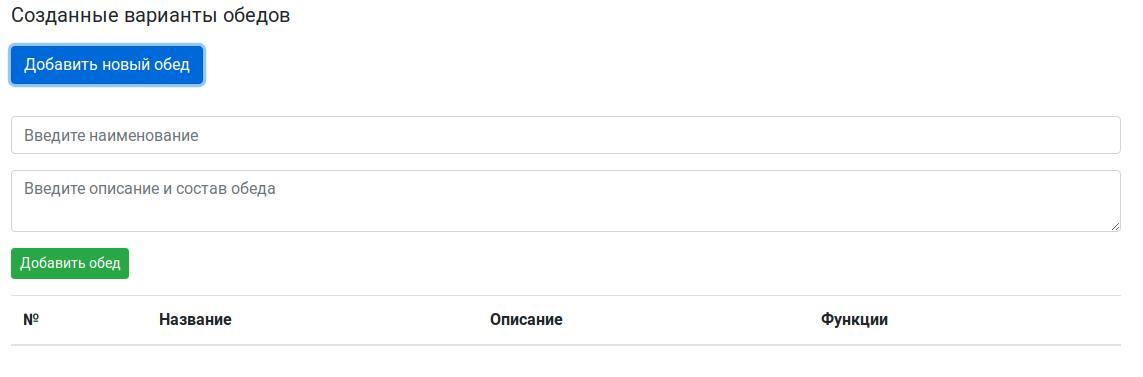
\includegraphics[width=1\linewidth]{015}}
\caption{Страница создания обедов}
\label{fig:image15}
\end{figure}

В открывшейся выпадающей форме необходимо ввести название комплекса обеда и его краткое описание\footnote{Обратите внимание, что форма ввода описания обеда динамическая и может расширяться, если не хватает места. Для этого нужно подцепить ее курсором за правый нижний край и потянуть вниз.}.

\begin{figure}[h]
\center{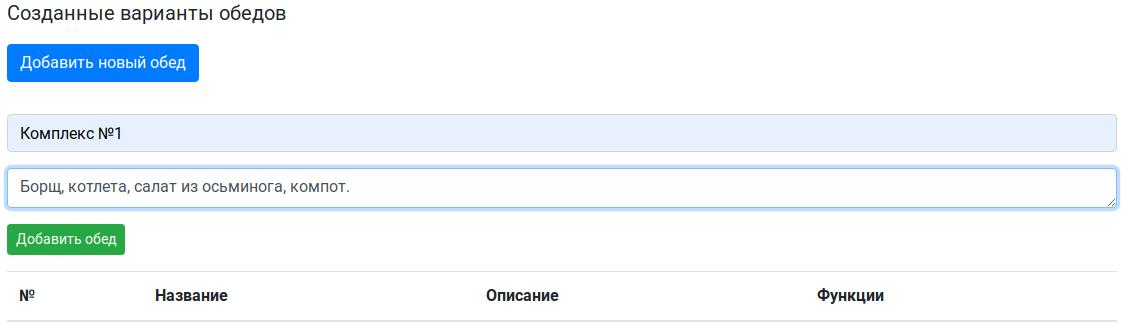
\includegraphics[width=1\linewidth]{016}}
\caption{Добавление нового обеда}
\label{fig:image16}
\end{figure}

Обратите внимание, что оба поля должны быть обязательно заполнены. Если хотя бы одно из них не заполнено, при попытке сохранить созданный обед система выдаст ошибку.

\begin{figure}[h]
\center{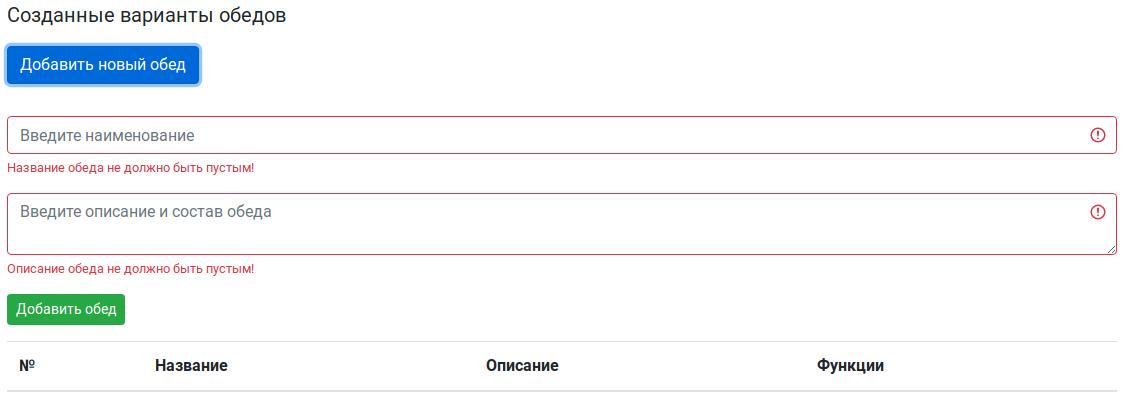
\includegraphics[width=1\linewidth]{017}}
\caption{Ошибка в добавлении обеда}
\label{fig:image17}
\end{figure}

Для сохранения введенных данных необходимо нажать кнопку \textbf{<<Добавить обед>>} в нижней части формы. При успешном добавлении произойдет переадресация на страницу обедов, в таблице которой появится созданный обед. Обратите внимание на столбец \textbf{№} - это системный идентификационный номер обеда, сгенерированный автоматически. В случае одинаковых названий обедов его можно использовать для их визуального различия.

\begin{figure}[h]
\center{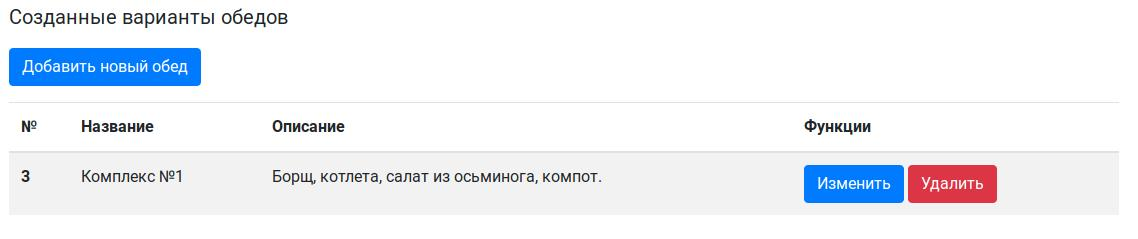
\includegraphics[width=1\linewidth]{018}}
\caption{Добавленный обед в таблице}
\label{fig:image18}
\end{figure}

\subsubsection{Изменение созданного обеда}

Для изменения уже созданного обеда необходимо нажать на кнопку \textbf{<<Изменить>>} в правой части строки обеда в таблице обедов. В открывшейся форме нужно подправить необходимые данные, после чего нажать кнопку \textbf{<<Изменить обед>>}.

\begin{figure}[h]
\center{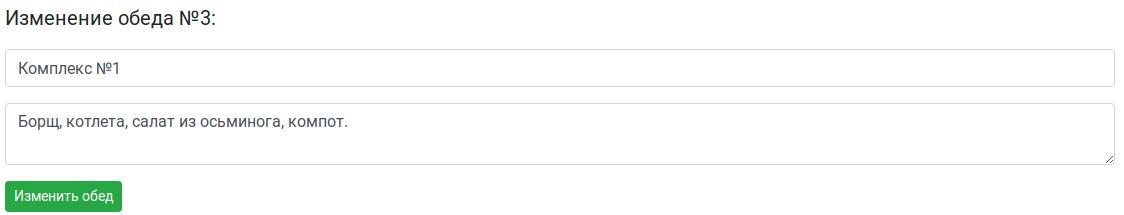
\includegraphics[width=1\linewidth]{019}}
\caption{Страница изменения обеда}
\label{fig:image19}
\end{figure}

Оба поля должны быть обязательно заполнены. В противном случае возможно появление сообщения об ошибке.

\begin{figure}[h]
\center{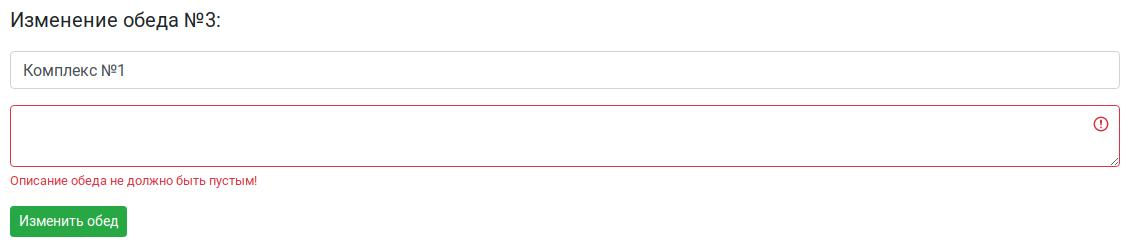
\includegraphics[width=1\linewidth]{020}}
\caption{Ошибка изменения обеда}
\label{fig:image20}
\end{figure}

\subsection{Настройка обедов по датам}

После успешного создания нескольких вариантов обедов их необходимо присвоить конкретным датам. На каждую дату можно присвоить два обеда, чтобы пользователи могли осуществить выбор. Настройка осуществляется на странице \textbf{<<Настройка обедов по датам>>}.

\begin{figure}[h]
\center{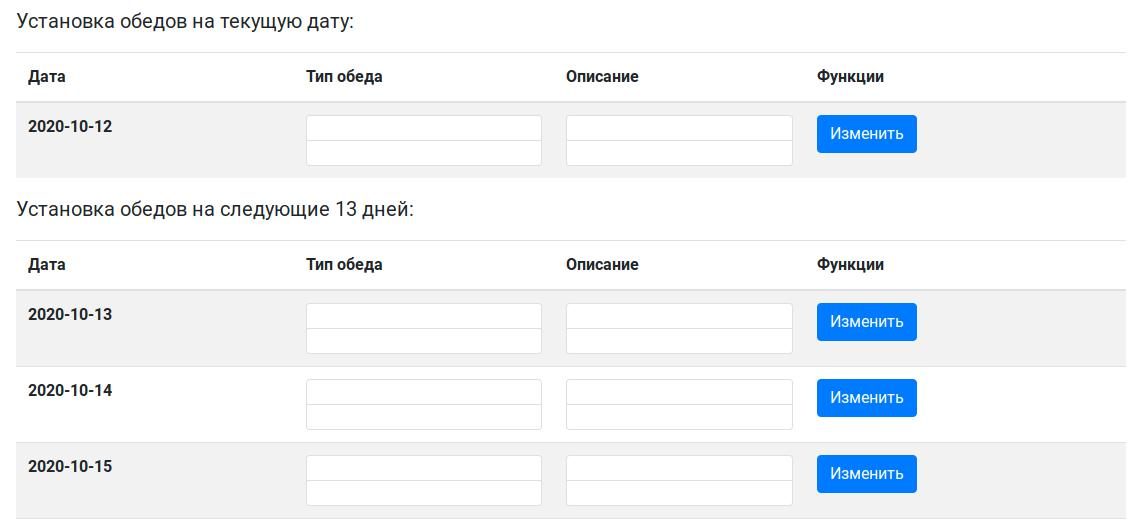
\includegraphics[width=1\linewidth]{021}}
\caption{Страница настроек обедов по датам}
\label{fig:image21}
\end{figure}

\textbf{\textit{Обратите внимание, что настроить обеды можно только на 14 дней, начиная с текущей даты!}} Предыдущие параметры удаляются из базы данных.

На странице настроек все данные отображаются в виде таблицы, содержащей следующие столбцы: дата, наименование обеда, его краткое описание и функции. Для присвоения обеда на определенную дату необходимо нажать кнопку \textbf{<<Изменить>>} в разделе функций.

\begin{figure}[h]
\center{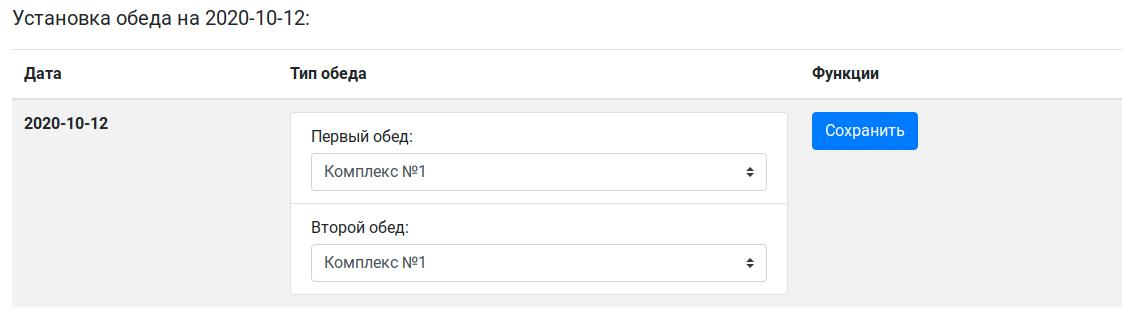
\includegraphics[width=1\linewidth]{022}}
\caption{Присвоение обедов определенной дате}
\label{fig:image22}
\end{figure}

На каждую дату можно выбрать два обеда: первый и второй варианты. Для присвоение первому или второму варианту конкретного обеда необходимо нажать на выпадающий список под соответствующей надписью и выбрать один из ранее созданных обедов.

\begin{figure}[h]
\center{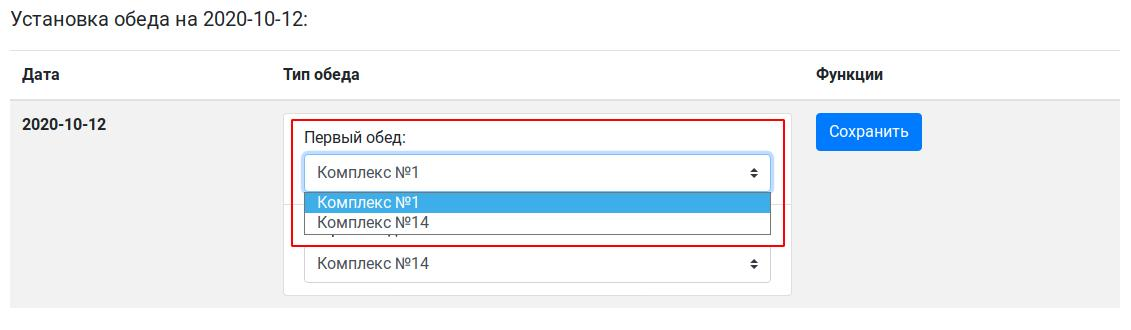
\includegraphics[width=1\linewidth]{023}}
\caption{Выбор ранее созданного обеда}
\label{fig:image23}
\end{figure}

После того, как оба обеда будут выбраны, необходимо нажать кнопку \textbf{<<Сохранить>>}, в результате чего настройки будут сохранены, а браузер будет снова перенаправлен на страницу настроек обедов по датам.

\begin{figure}[h]
\center{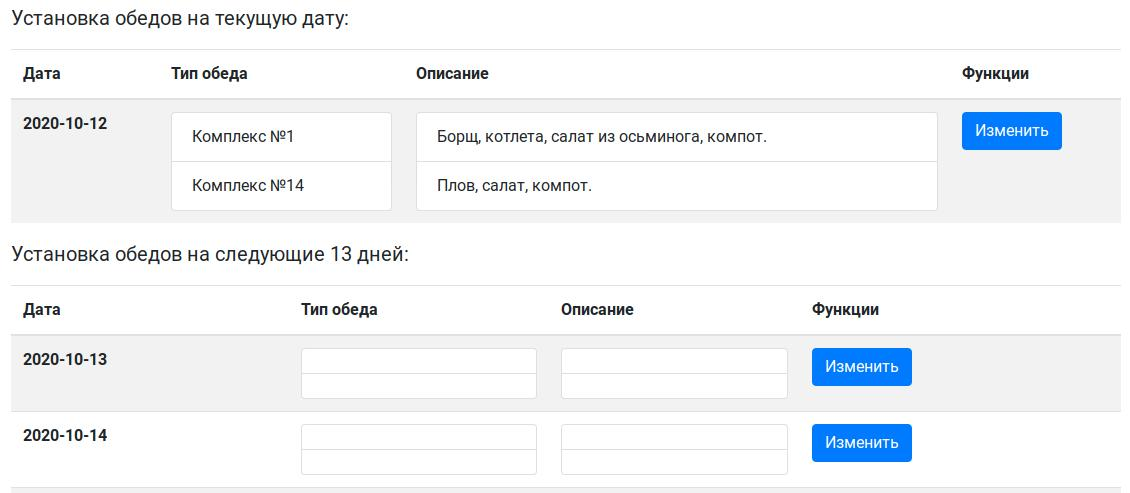
\includegraphics[width=1\linewidth]{024}}
\caption{Настроенный обед на текущую дату}
\label{fig:image24}
\end{figure}

Изменение заданных обедов происходит точно так же по нажатию кнопки \textbf{<<Изменить>>}.

\section{Выбор обедов простым пользователем}

Для простого пользователя доступно только одно меню - \textbf{<<Мои обеды>>}. Для удобства далее будет рассмотрена только мобильная версия приложения.

\begin{figure}[h]
\begin{minipage}[h]{0.49\linewidth}
\center{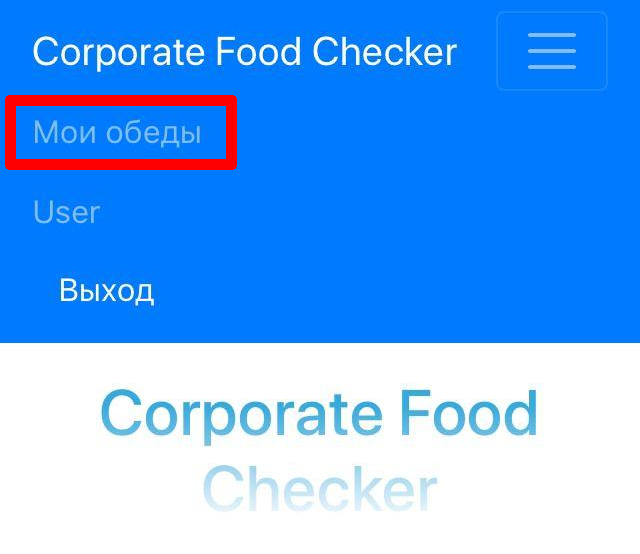
\includegraphics[width=0.5\linewidth]{025} \\ а)}
\end{minipage}
\hfill
\begin{minipage}[h]{0.49\linewidth}
\center{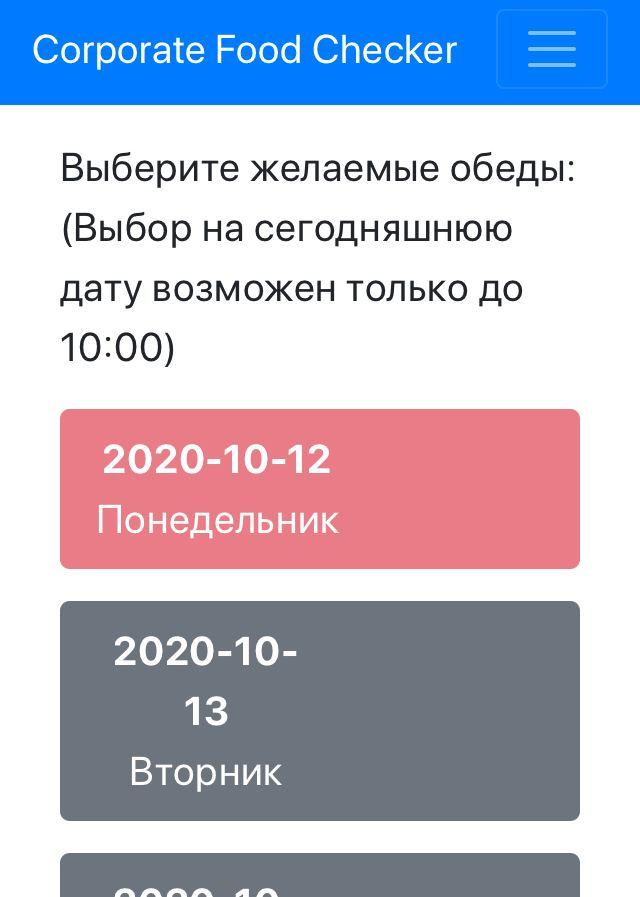
\includegraphics[width=0.5\linewidth]{026} \\ б)}
\end{minipage}
\caption{\textbf{<<Мои обеды>>}}
\label{fig:image26}
\end{figure}

Для удобства использования на маленьких экранах можно перевернуть телефон в ландшафтный режим.

При переходе на страницу пользователю будут показаны активные элементы управления, соответствующие каждому из 14 предстоящих дней. 

\begin{figure}[h!]
\center{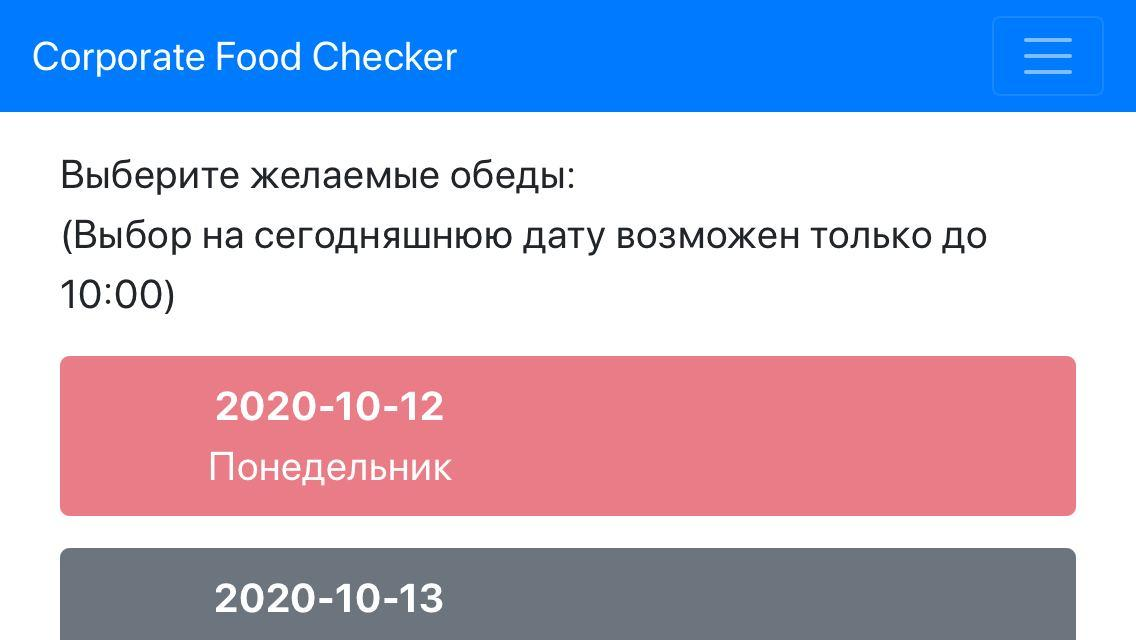
\includegraphics[scale=0.41]{027}}
\caption{Страница в ландшафтном режиме}
\label{fig:image27}
\end{figure}

\textbf{Обратите внимание! Выбор обеда на текущую дату доступен только до 10.00 утра!}

Расцветка элементов управления имеет следующие градации:

\begin{itemize}
\setlength{\itemsep}{-2mm}
	\item \textbf{Серый} - пользователь еще не выбрал обед на эту дату;
	\item \textbf{Синий} - пользователь выбрал обед на эту дату;
	\item \textbf{Красный} - (применимо только к текущей дате) изменить можно было только до 10:00 утра;
\end{itemize}

Для выбора обеда на дату выберите нужную, щелкнув (тапнув) по соответствующему элементу управления. На открывшейся странице будут показаны оба доступных варианта обеда с названием и описанием. Для выбора одного конкретного необходимо кликнуть (тапнуть) по выпадающему списку ниже и выбрать один из доступных вариантов.

\begin{figure}[h]
\begin{minipage}[h]{0.49\linewidth}
\center{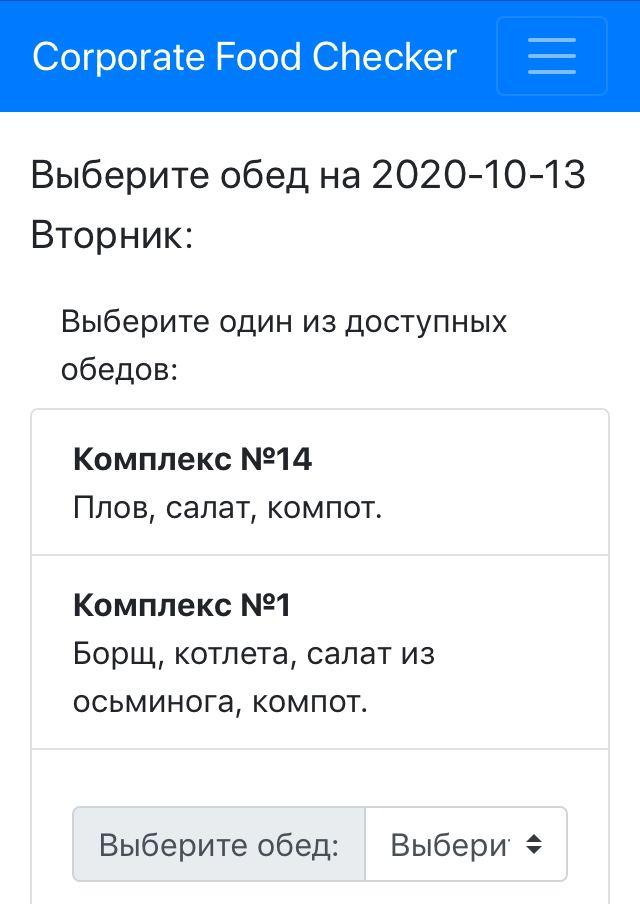
\includegraphics[width=1\linewidth]{028} \\ а)}
\end{minipage}
\hfill
\begin{minipage}[h]{0.49\linewidth}
\center{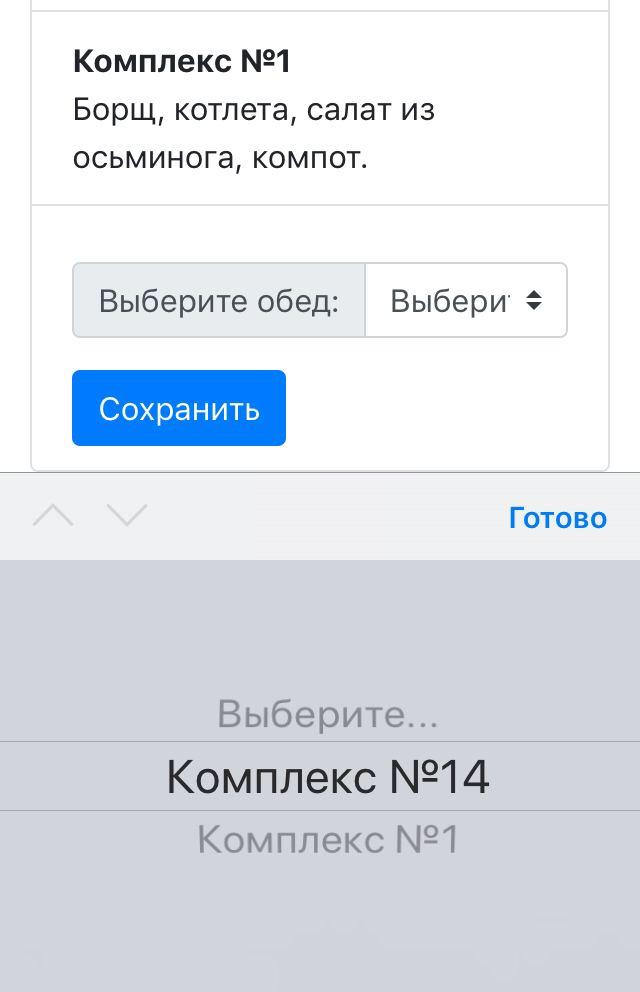
\includegraphics[width=1\linewidth]{029} \\ б)}
\end{minipage}
\caption{Выбор обеда}
\label{fig:image29}
\end{figure}

Для сохранения выбора необходимо нажать кнопку \textbf{<<Сохранить>>}, после чего произойдет перенаправление обратно на страницу <<Мои обеды>>. Выбранный обед появится на соответствующем элементе управления, а цвет последнего сменится на синий.

\begin{figure}[h!]
\center{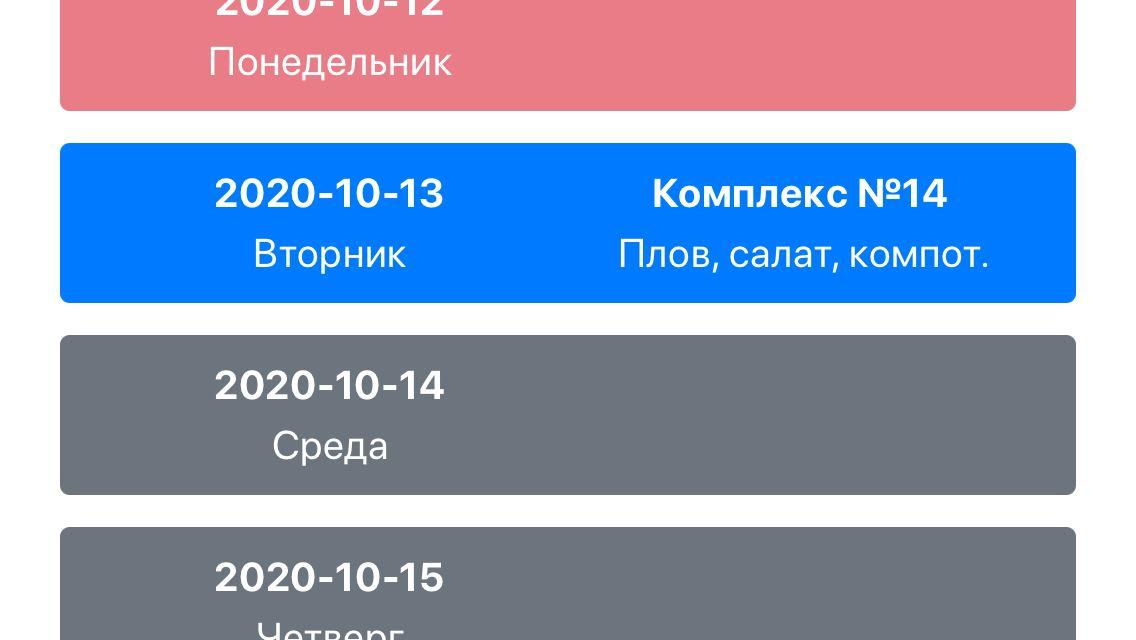
\includegraphics[scale=0.41]{030}}
\caption{Выбранный обед}
\label{fig:image30}
\end{figure}

В случае, если администратор системы еще не задал обеды на соотетствующие даты, будет показана ошибка.

\begin{figure}[h!]
\center{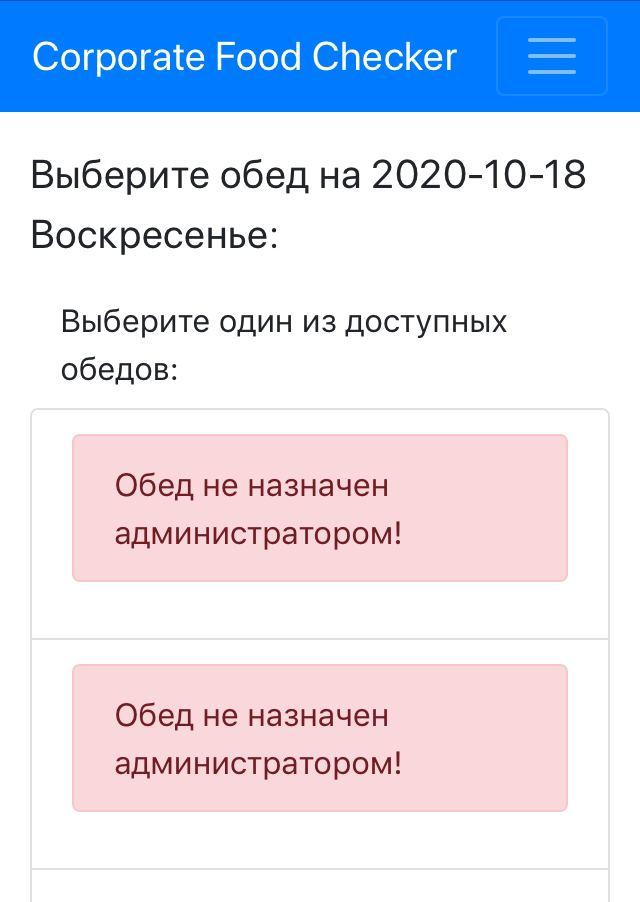
\includegraphics[scale=0.5]{031}}
\caption{Обед еще не назначен на эта дату}
\label{fig:image31}
\end{figure}

\section{Просмотр статистики по выбранным обедам}

Просмотр статистики по обедам \textbf{доступен только администратору системы}. Для просмотра необходимо перейти на страницу \textbf{<<Таблица обедов>>}, где в виде таблицы будут представлены выбранные пользователями обеды и их количество на каждую из дат.

\begin{figure}[h]
\center{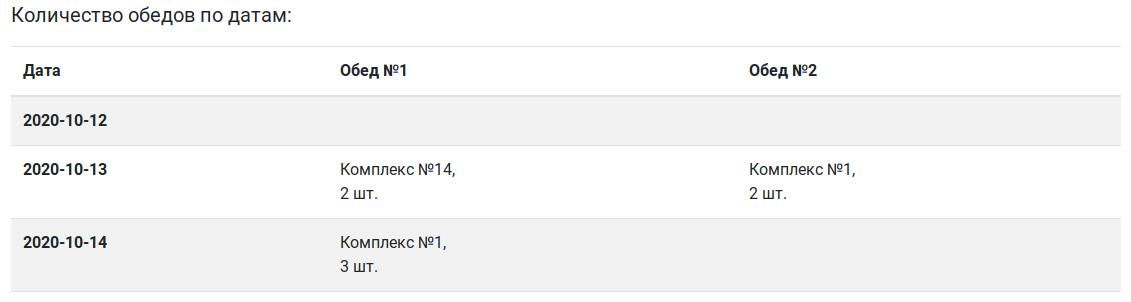
\includegraphics[width=1\linewidth]{032}}
\caption{Таблица обедов}
\label{fig:image32}
\end{figure}

\newpage
\section{О программе}

Разработчик приложения: Нежберт Константин.

По всем вопросам и предложениям обращаться на электронную почту \\
\textbf{zhbert@yandex.ru}.

\end{document}  % КОНЕЦ ДОКУМЕНТА !